\subsection{Point estimate}
\label{sec:etas-point}

In a perfect world, it would be possible to predict precisely how long it would take a bus to arrive at a stop, and display this single number to passengers. Alas, as we saw in \cref{cha:prediction}, this is not a perfect world, and arrival time prediction inherently comes with significant uncertainty. Yet we still need to decide on the best single value to use as a point estimate of arrival time, since much of the infrastructure currently available only allows this. We also want to examine if it is possible to come up with a single statistic that performs well---on average---and, more importantly, better than the currently deployed method.





\begin{knitrout}
\definecolor{shadecolor}{rgb}{0.969, 0.969, 0.969}\color{fgcolor}\begin{figure}

{\centering 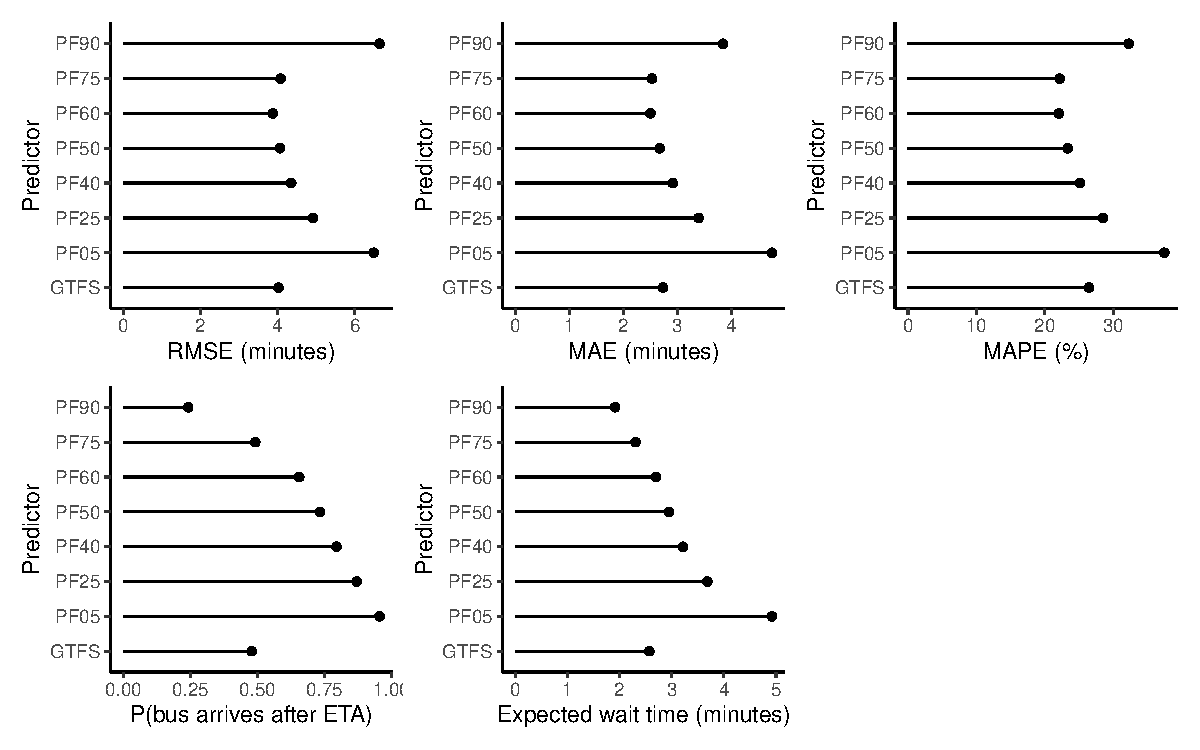
\includegraphics[width=\textwidth]{figure/eta_overall_results-1} 

}

\caption[ETA stuff]{ETA stuff}\label{fig:eta_overall_results}
\end{figure}


\end{knitrout}


We calculated, for all stops, trips, and times, a range of arrival times quantiles ($q \in \{0.05, 0.25, 0.5, 0.6, 0.6, 0.75, 0.9\}$), and for each computed the \gls{rmse}, the probability of catching the bus given you arrive at the stated \gls{eta}, $\Pcatch$, and the expected waiting time given you catch the bus, $\Ewait$. The results are displayed in \cref{fig:eta_overall_results}, along with the same values computed used the \gls{gtfs} arrival time estimates. For the particle filter, the lowest \gls{rmse} value is achieved when using the 60\% quantile, which obtains a 66\% probability of the bus arriving after the \gls{eta} and an expected waiting time of 2.7~minutes. The coverage of the quantiles are being overestimated---we would expect the 60\% quantile to have an approximately 40\% success rate---which indicates that the current implementation of the particle filter is underestimating arrival times.


\begin{knitrout}
\definecolor{shadecolor}{rgb}{0.969, 0.969, 0.969}\color{fgcolor}\begin{figure}

{\centering 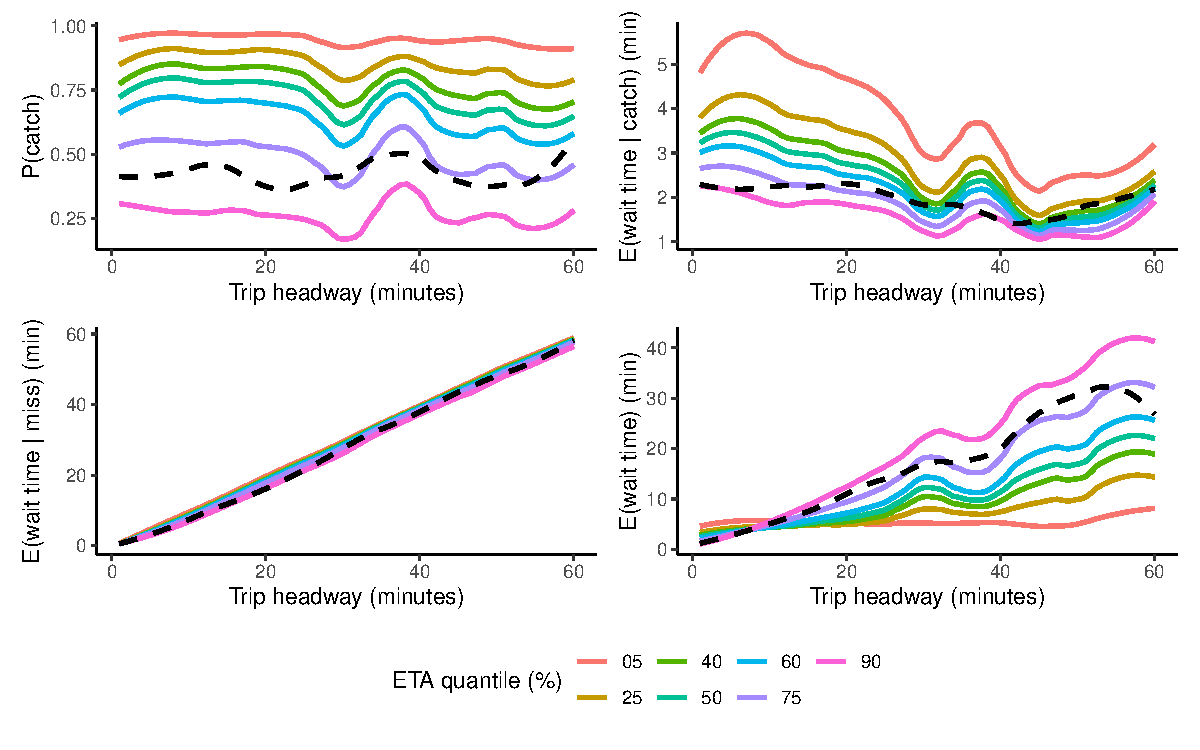
\includegraphics[width=\textwidth]{figure/eta_headway_results-1} 

}

\caption[More ETA stuff]{More ETA stuff}\label{fig:eta_headway_results}
\end{figure}


\end{knitrout}

An important consideration is the cost of missing the bus. For each trip, we computed the scheduled time between the current trip and the subsequent one (which is termed \emph{headway}) to compute the expected waiting time if the bus arrives \emph{before} the predicted time. That is, if a bus is predicted to arrive in 5~minutes, but actually arrives in 3, and the time until the next bus (servicing the same trip) is 10~minutes, then the expected waiting time will be $10-5=5$~minutes (assuming the passenger arrives in 5~minutes). This \emph{headway} is an essential component to prediction cost.

The total expected wait time can be conditioned on whether or not the bus was caught,
\begin{equation}
\label{eq:eta_wait_conditional}
\begin{split}
\E{\text{wait}} &=
  \Pr{\text{catch}} \E{\text{wait}|\text{catch}} +
  (1 - \Pr{\text{catch}}) \E{\text{wait}|\text{miss}} \\
  &= \Pr{A \geq a} \E{A - a | A \geq a} +
  \Pr{A < a}\E{\text{headway} - a + A | A < a}
\end{split}
\end{equation}
where $a$ is the estimated arrival time, and $A$ is the actual. For simplicity, we assume headway is maintained (which it is not, \cite{})---that is, if a bus has 20~minute frequency and you miss the bus by 5~minutes, your expected waiting time is 15~minutes.

\Cref{fig:eta_headway_results} shows the values of $\Pcatch$, $\Ecatch$, $\Emiss$, and $\Ewait$ by headway (rounded down, in minutes). Capture probability is not so affected by headway, though it decreases slightly for longer headways. In contrast, expected wait times are very much affected. Most unexpectedly, $\Ecatch$ decreases with headway, which could be caused by a higher proportion of short headway at peak times when traffic is more congested, leading to more uncertainty (so the quantiles are more dispersed), or the buses take longer than expected. For $\Emiss$, the expected wait time is not unexpectedly strongly correlated with headway. Overall, the difference in $\Ewait$ between predictors is negligible for headways less than 10~minutes, after which time differences appear. Low frequency routes should prefer a low quantile to reduce the chance of missing the bus.


We did not examine time-until-arrival, which we saw in the previous chapter explained a lot of the variation in predictor performance. We would expect a similar result here, so if one wanted to develop a predictor based on both headway and time until arrival, that would be straightforward enough. However, it is clear that the choice of predictor is tightly linked with the cost of a bad prediction: is waiting at the bus stop too long more costly than missing it altogether?
